%!TEX root = paper.tex

\subsection{Concretization}

We have discussed Spack's internal software DAG model, and we have shown
how the spec syntax can be used to quickly specify a partially constrained
software DAG.  We say such a DAG is {\it abstract}, i.e. it could potentially describe
more than one unique software configuration. Before Spack builds a spec, it
must ensure the folioing conditions:
\begin{enumerate}
\item No package in the spec DAG is missing dependencies.
\item No package in the spec DAG is virtual.
\item All parameters are set for all packages in the DAG.
\end{enumerate}
If a spec meets all of these criteria, we say it is {\it concrete}.
The central component of the Spack build that allows it to reduce a 
highly unconstrained abstract description to a concrete build, is
called {\it concretization}.

\begin{figure*}
	\centering
	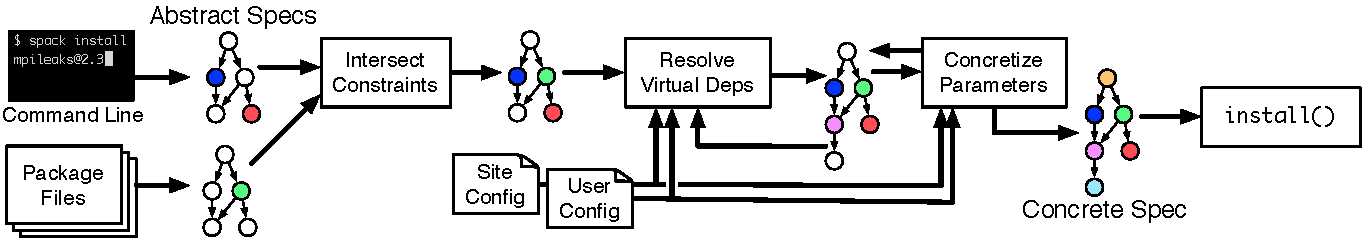
\includegraphics[width=\textwidth]{figs/concretization.pdf}
	\caption{
		Concretization resolves an abstract spec DAG into a concrete spec that can be installed.
		\label{fig:concretization}
	}
\end{figure*}

Spack's concretization algorithm is shown in Figure~\ref{fig:concretization}.
The process starts when a user invokes {\tt spack install} and requests that
a spec be built.  Spack converts the user's spec to an abstract spec DAG.
It then builds a {\it separate} spec DAG for any constraints that are encoded
in directives in package files. 

Spack intersects the constraints of the two DAGs package by package.  It checks
each parameter for inconsistencies.  Inconsistencies can arise if, for example,
the user inadvertently requests two versions of the same package, or if a
package file explicitly requests a different version from what the user requested.
Likewise, if the package and the user specified different compilers, variants,
or platforms for particular packages, this will cause the user to be notified
of the contradiction. If the user or package specified version ranges, they are
intersected, and if the ranges do not overlap, an error will be raised.
When the intersection succeeds, Spack has a single spec DAG with the merged
constraints of the user and the package files.  

The next part of the process is iterative.
If any node in the DAG is a virtual dependency, spack replaces it with with a
suitable concrete interface provider.  It does this by building a reverse
index from virtual packages to providers using the {\tt provides when} 
directives discussed in Section~\ref{sec:virtual}. If multiple providers
could satisfy the constraints on the virtual spec, 
Spack will consult site and user policies to select the ``best'' possible
provider.  The selected provider may {\it itself} have virtual dependencies,
so Spack repeats this process until there are no more virtual packages
in the DAG.

With the now non-virtual DAG, Spack again consults site and user preferences for 
variants, compilers, and versions to resolve any remaining abstract nodes.
Adding a variant {\it may} cause a package to depend on more libraries. For example,
if the site default behavior is to have a particular package build with {\tt +python},
and this causes it to depend on Python libraries, then the cycle begins again.
Spack currently avoids cycles by using a greedy algorithm.  It will not backtrack and
try other options if the first policy choice leads to an inconsistency.  In future
work we will investigate adding a SAT solver to Spack's concretization process to
handle these cases, but in practice, we have found complex policy interactions to be
very rare.

When the process completes, it outputs a fully concrete Spec DAG.  An example 
concrete DAG with architectures, compiler, versions, and variants, and all 
dependencies resolved is shown in Figure~\ref{fig:specs-mpileaks-concrete}.
The concrete DAG fulfills Spack's guarantees.


\begin{figure}
	\centering
	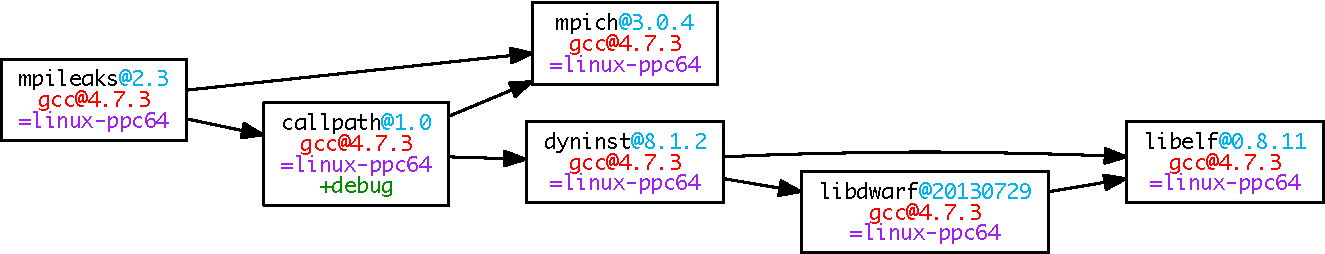
\includegraphics[width=\columnwidth]{specs/mpileaks-concrete.pdf}
	\caption{
		Concretized version of specs from Figure~\ref{fig:specs-mpileaks}.
		\label{fig:specs-mpileaks-concrete}
	}
\end{figure}

At install time, Spack constructs a package object for each node in the spec DAG
and traverses the DAG in a bottom-up fashion.  At each node, it invokes the package's
{\tt install()} method, using a sub-DAG rooted at the package to be installed as the {\tt spec}
parameter to {\tt install()}. Package maintainers are responsible for examining the 
concrete spec and adjusting the build if necessary.

In our experience, much complexity in build scripts arises from the need for the script to
query the environment and disambiguate complex environment settings.  If the build process is
ill-defined, and the desired build configuration is often nonspecific, and it is these
ambiguities that cause many build systems to fall over when faced with too many configuration
options.

In spack, build scripts are free from this concern, because the package author
is guaranteed that a package's build spec is concrete at {\tt install()} time.
There is thus no need to perform complicated state checks in spack build scripts;
the {\tt spec} itself has the full configuration.  Other multi-configuration systems like Nix, 
EasyBuild, and hashdist require the package author to write a mostly concrete build
spec up front, and there is no way to set concretization policies in the way that Spack
allows them.  We believe that this puts undue burden on the package author.  It also makes
the task of separating site policies from user policies difficult.













